% !TeX root= FEM
\section{Quadrature}

\subsection{Motivation}
We want to compute Integrals of the form:
\begin{align*}
	\int \limits_\Omega f(x) \diff x.
\end{align*}
\underline{Problems}
\begin{itemize}
	\item primitive doesn't always exist ($F\colon F'=f$)
	\item analytic computation on PC problematic
\end{itemize}

 \underline{special case: FEM}
 \begin{itemize}
 	\item 
 	\begin{equation*}
 		A_{ij} = \int \limits_\Omega \nabla \varphi_j \cdot \nabla \varphi_i \diff x
 	\end{equation*}
 	\item no closed form of $\varphi_i$ on $\Omega$
 	\item philosophical: FEM is just an approximation
 \end{itemize}

$\implies$ Aim: Approximate $\int \limits_\Omega f(x) \diff x$

\underline{Approach}
\begin{equation*}
	\int \limits_\Omega f(x) \diff x \approx \displaystyle \sum_{k=1}^{N_Q} w_k f(x_k)
\end{equation*}
with $w_k \in \R$ (weights) and $x_k \in \Omega$ (points/nodes). Together the set $\{(w_k,x_k)\}$ is called quadrature rule.\\
\underline{Questions:}
\begin{enumerate}[label=\arabic*)]
	\item Do I need a quadrature rule for every $\Omega$?
	\item How do I choose $\{(w_k,x_k)\}$?
	\item How do I measure the quality of approximation?
\end{enumerate}

\subsection{Transformation}
Integral Transformation, $\hat{\Omega}, \Phi(\hat{\Omega}) = \Omega$
\begin{align}
	\int \limits_{\Phi(\Omega)}  f(y) \diff y &= \int \limits_{\hat{\Omega}} f(\Phi(y)) |\det(D\Phi(x))| \diff x \\
	&\approx \displaystyle \sum^{N_Q}_{k=1} f(\underbrace{\Phi(x_k)}_{\in \Omega}) \underbrace{|\det(D\Phi)|}_{\in \R} \diff
\end{align}
Note that in our case $\Phi$ is an affine linear function and thus $D\Phi$ does not depend on $x$.
$\{(|\det(D\Phi)|w_k,\Phi(x_k))\}$ is a quadrature rule on $\Omega$.
\subsection{Exactness}
Aim: measure the approximation quality\\
\underline{Notation}
\begin{itemize}
	\item $\hat{\Omega}$, $\{(w_k,x_k)\}$ quadrature rule on $\hat{\Omega}$
	\item $I(f):= \int \limits_{\hat{\Omega}} f(x) \diff x$
	\item $Q(f):= \displaystyle \sum_{k=1}^{N_Q} w_k f(x_k)$
	\item $\mathbb{P}_m(\hat{\Omega}) \dots $ polonomials of degree $\leq m$ on $\hat{\Omega}$
\end{itemize}
\begin{definition}
	A quadrature rule is exact of order $m$ $\iff$
	\begin{equation*}
		I(f)= Q(f) \qquad \forall p\in \mathbb{P}_m(\hat{\Omega})
	\end{equation*}
	and there exists $p\in \mathbb{P}_{m+1}$ s.t. $I(f)\neq Q(f)$
\end{definition}
\begin{lemma_}
	exact of order $m$ $\iff$ exact for $\{1,x,x^2,\dots,x^m \}$
\end{lemma_}

\begin{thrm}
	(1D): a quadrature rule with $N_Q$ points has a degree of exactness $\leq 2N_Q -1$
\end{thrm}

\subsection{Optimal Quadrature Rules}
\underline{Gaussian Quadrature Rules}: Aim: Exactness $2N_Q-1$
\vspace{0.5cm}\\
\underline{Dimension 1}, Intervall [0,1]\\
$N_Q = 1$ $\implies$ exact for $\{1,x\}$
\begin{equation*}
	Q(f)= w_1f(x_1)
\end{equation*}
\begin{align*}
	w_1 &= Q(1) = I(1)= 1 &\implies & w_1 = 1\\
	w_1x_1 &= Q(x) = I(x)= \frac{1}{2} &\implies & x_1 = \frac{1}{2}
\end{align*}

$N_Q = 2$ $\implies$ exact for $\{1,x,x^2.x^3\}$
\begin{equation*}
	Q(f)= w_1f(x_1) + w_2f(x_2)
\end{equation*}
\begin{align*}
\begin{rcases}
	1 &= I(1)=Q(1)  \\
	\frac{1}{2} &= I(x)= Q(x)  \\
	\frac{1}{3}&=I(x^2)= Q(x^2) \\
	\frac{1}{4}&=I(x^3)= Q(x^3)
\end{rcases} \implies w_1=w_2= \frac{1}{2}, x_{1,2} = \frac{\sqrt{3}\pm 1}{2\sqrt{3}}
\end{align*}
\begin{figure}[H]
	\center
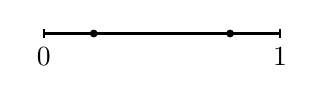
\begin{tikzpicture}[scale=3]

        \draw[thick] (0,0) -- ++(1,0);
        \draw[thick] (0,-0.02) -- ++(0,0.04);
        \draw[thick] (1,-0.02) -- ++(0,0.04);

        \filldraw (0.788675,0) circle (0.4pt);
        \filldraw (0.211325,0) circle (0.4pt);
        \node at (0,-0.02) [below] {0};
        \node at (1,-0.02) [below] {1};

\end{tikzpicture}

\caption{Visualisation of nodes in $\hat{\Omega}  = [0,1] $}
\label{ch_quad_nodes_intervall}

\end{figure}
\underline{Dimension 2}\\
$\hat{\Omega} = [0,1]\times [0,1]$ $\implies \{\{x_k\}\times\{x_k\} \}$ quadrature points on $\hat{\Omega}$
\begin{figure}[H]
	\center
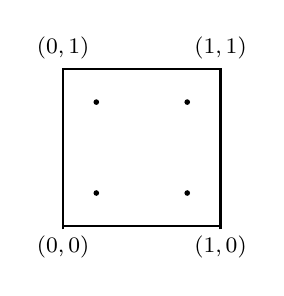
\begin{tikzpicture}[scale=2]

\draw[thick] (0,0) -- ++(1,0) -- ++(0,1) -- ++(-1,0)--cycle;
\draw[thick] (0,-0.02) -- ++(0,0.04);
\draw[thick] (1,-0.02) -- ++(0,0.04);

\filldraw (0.788675,0.211325) circle (0.4pt)
		  (0.788675,0.788675) circle (0.4pt)
	      (0.211325,0.788675) circle (0.4pt)
		  (0.211325,0.211325) circle (0.4pt);
\fill[black,font=\footnotesize] (0,0)         node[below] {$(0,0)$}
								(0,0) ++(0,1) node[above] {$(0,1)$}
								(0,0) ++(1,1) node[above] {$(1,1)$}
								(0,0) ++(1,0) node[below] {$(1,0)$};

\end{tikzpicture}

\caption{Visualisation of nodes in $\hat{\Omega}  = [0,1] \times [0,1] $}
\label{ch_quad_nodes_quadrat}

\end{figure}
$\hat{\Omega} = \hat{T}$\\
First Approach: transform $[0,1]\times [0,1]$ to $\hat{T}$.
\begin{figure}[H]
\center
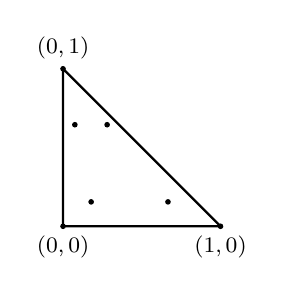
\begin{tikzpicture}[scale=2]

        \draw[thick] (0,0) -- ++(0,1) -- ++(1,-1)--cycle;
        \filldraw (0,0)         circle (0.4pt);
        \filldraw (0,0) ++(1,0) circle (0.4pt);
        \filldraw (0,0) ++(0,1) circle (0.4pt);
        \fill[black,font=\footnotesize] (0,0)         node[below] {$(0,0)$}
                                        (0,0) ++(0,1) node[above] {$(0,1)$}
                                        (0,0) ++(1,0) node[below] {$(1,0)$};
        \filldraw (0.666390, 0.155051) circle (0.4pt);
        \filldraw (0.280020, 0.644949) circle (0.4pt);
        \filldraw (0.178559, 0.155051) circle (0.4pt);
        \filldraw (0.075031, 0.644949) circle (0.4pt);
\end{tikzpicture}
\caption{Visualisation of nodes in $\hat{T}$(order 3)}\label{ch_quad_nodes_T_hat}

\end{figure}
Second Approach: derive optimal rules on $\hat{T}$\\
$N_Q = 1$ $\implies$ exact for $\{1,x,y\}$
\begin{equation*}
Q(f)= w_1f(x_1,y_1)
\end{equation*}
\begin{align*}
\begin{rcases}
\frac{1}{2}&= I(1)= Q(1) = w_1  \\
\frac{1}{6}&= I(x)= Q(x) = w_1x_1  \\
\frac{1}{6}&= I(y)= Q(y) = w_1y_1\\
\end{rcases} \implies w_1= \frac{1}{2}, x_1=y_1 = \frac{1}{3}
\end{align*}
something is probably wrong here\\
$N_Q = 3$ $\implies$ exact for $\{1,x,y,x^2,y^2\}$
\begin{equation*}
Q(f)= w_1f(x_1,y_1) + w_2f(x_2,y_2) + w_3f(x_3,y_3)
\end{equation*}
\begin{align*}\implies
\begin{cases}
(x_1,y_1)&= (1/6,1/6),  \qquad w_1= 1/6\\
(x_2,y_2)&= (2/3,1/6),  \qquad w_2= 1/6\\
(x_3,y_3)&= (1/6,2/3),  \qquad w_3= 1/6
\end{cases} 
\end{align*}
$N_Q = 4$ $\implies$ exact for $\{1,x,y,x^2,y^2,x^3,y^3\}$
\begin{equation*}
Q(f)= w_1f(x_1,y_1) + w_2f(x_2,y_2) + w_3f(x_3,y_3) + w_4f(x_4,y_4)
\end{equation*}
\begin{align*}\implies
\begin{cases}
(x_1,y_1)&= (1/3,1/3),  \qquad w_1= \frac{-27}{96}\\
(x_2,y_2)&= (2/3,1/6)  \\
(x_3,y_3)&= (1/6,2/3),  \qquad w_{2,3,4}= \frac{25}{96}\\
(x_4,y_4)&= (1/6,2/3)
\end{cases} 
\end{align*}
\begin{figure}[H]
	\center
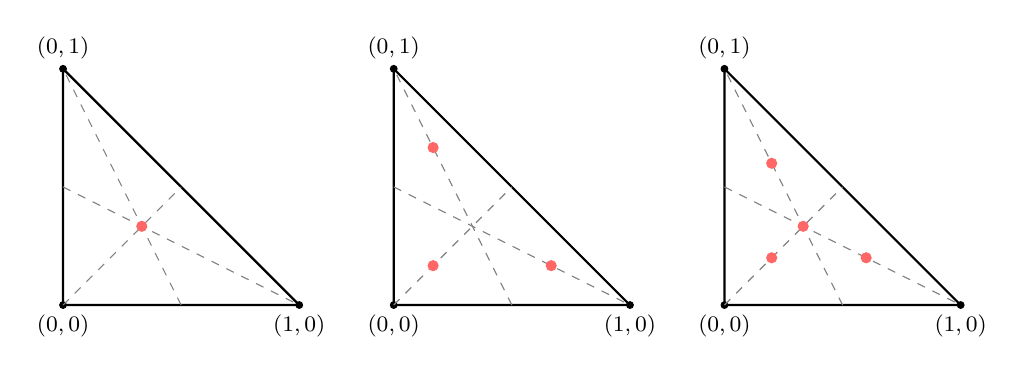
\begin{tikzpicture}[scale=3]
		
		\def \xone{0};
		\def \yone{0};		
		% first rectangle
		\coordinate (A) at (\xone,\yone);
		
        \draw[thick] (A) -- ++(0,1) -- ++(1,-1)--cycle;
        \filldraw (A)         circle (0.4pt);
        \filldraw (A) ++(1,0) circle (0.4pt);
        \filldraw (A) ++(0,1) circle (0.4pt);
        \fill[black,font=\footnotesize] (A)         node[below] {$(0,0)$}
                                        (A) ++(0,1) node[above] {$(0,1)$}
                                        (A) ++(1,0) node[below] {$(1,0)$};
        \draw[dashed,gray] (A) ++(0,1/2) -- ++(1,-1/2);
        \draw[dashed,gray] (A) -- ++(1/2,1/2);
        \draw[dashed,gray] (A) ++(1/2,0) -- ++(-1/2,1);
        
        \filldraw[red!60] (A)++(1/3, 1/3) circle (0.6pt);
        
        
        % second rectangle
        \coordinate (A1) at (\xone + 1.4,\yone);
        
        \draw[thick] (A1) -- ++(0,1) -- ++(1,-1)--cycle;
        \filldraw (A1)         circle (0.4pt);
        \filldraw (A1) ++(1,0) circle (0.4pt);
        \filldraw (A1) ++(0,1) circle (0.4pt);
        \fill[black,font=\footnotesize] (A1)         node[below] {$(0,0)$}
								        (A1) ++(0,1) node[above] {$(0,1)$}
        								(A1) ++(1,0) node[below] {$(1,0)$};
        
        \draw[dashed,gray] (A1) ++(0,1/2) -- ++(1,-1/2);
        \draw[dashed,gray] (A1) -- ++(1/2,1/2);
        \draw[dashed,gray] (A1) ++(1/2,0) -- ++(-1/2,1);
        
        \filldraw[red!60] (A1)++(1/6, 1/6) circle (0.6pt);
        \filldraw[red!60] (A1)++(2/3, 1/6) circle (0.6pt);
        \filldraw[red!60] (A1)++(1/6, 2/3) circle (0.6pt);
        
        % third rectangle
        \coordinate (A2) at (\xone + 2.8,\yone);
        
        \draw[thick] (A2) -- ++(0,1) -- ++(1,-1)--cycle;
        \filldraw (A2)         circle (0.4pt);
        \filldraw (A2) ++(1,0) circle (0.4pt);
        \filldraw (A2) ++(0,1) circle (0.4pt);
        \fill[black,font=\footnotesize] (A2)         node[below] {$(0,0)$}
        								(A2) ++(0,1) node[above] {$(0,1)$}
 								        (A2) ++(1,0) node[below] {$(1,0)$};
        
        \draw[dashed,gray] (A2) ++(0,1/2) -- ++(1,-1/2);
        \draw[dashed,gray] (A2) -- ++(1/2,1/2);
        \draw[dashed,gray] (A2) ++(1/2,0) -- ++(-1/2,1);
        
        \filldraw[red!60] (A2)++(1/3, 1/3) circle (0.6pt);
        \filldraw[red!60] (A2)++(1/5, 3/5) circle (0.6pt);
        \filldraw[red!60] (A2)++(1/5, 1/5) circle (0.6pt);
        \filldraw[red!60] (A2)++(3/5, 1/5) circle (0.6pt);
\end{tikzpicture}

\caption{Visualisation of other nodes in $\hat{T}$ for $N_Q =1,3,4$ (order 1,2,3)}
\label{ch_quad__other_nodes_T_hat}
\end{figure}
Note that in the above picture the dashed lines show the position of nodes for higher order quadrature rules.
%%TODO add picture for higher order secpnd approach